\chapter{PROGRAMAS Y HOJAS DE CÁLCULO}
\label{anx:programas}

Este anexo registra los programas, las versiones, los libros de cálculo y los guiones que respaldan los Capítulos~\ref{cap:diseno} y~\ref{cap:resultados}. Las rutas que comienzan con \texttt{evidencias/} se encuentran en la carpeta del informe; las demás, en \RepoProyecto, descrito en el Anexo~\ref{anx:portafolio}.

\section{Programas y guiones empleados}
\label{sec:programas-empleados}

La Tabla~\ref{tab:programas} relaciona cada programa con su uso y con sus archivos de respaldo.

\begingroup
\small\singlespacing
\setlength{\tabcolsep}{4pt}
\begin{longtable}{@{}>{\raggedright\arraybackslash}p{3.1cm}>{\raggedright\arraybackslash}p{4.6cm}>{\raggedright\arraybackslash}p{\dimexpr\textwidth-7.7cm-4\tabcolsep\relax}@{}}
\caption{Programas, versiones y archivos de respaldo}\label{tab:programas}\\
\toprule
\textbf{Programa} & \textbf{Uso} & \textbf{Archivos de respaldo}\\
\midrule\endfirsthead
\toprule
\textbf{Programa} & \textbf{Uso} & \textbf{Archivos de respaldo}\\
\midrule\endhead
\bottomrule\endlastfoot
SAP2000 24.2.0 & Análisis estructural del bastidor de tres apoyos sectoriales (corrida de referencia) & \path{evidencias/N3_R01/V5_2_N3_W6X9_R01.sdb}; \path{R01_SAP_ORIGINAL.xlsx}; \path{SHA256_EVIDENCIA_R01.txt}\\
FreeCAD 1.1.1 & Modelo CAD integrado, barridos de interferencia y exportación de vistas & \path{cad/integracion_R06/R06.1_centradores/cad/R061_K2M_V573_CANDIDATO.FCStd}; guion de vistas \path{images/cad/_render_vistas_freecad.py}\\
FreeCAD FEM con CalculiX 2.22 & Elementos finitos locales de los centradores U1, U2 y U3 & \path{estructural/integracion_R06/R06.1_centradores/resultados/k2m_v57/}\\
CalculiX 2.22 y guion Python & Modelo global del bastidor y corrección por alabeo con una parrilla de Vlasov & \path{estructural/integracion_R06/R06.1_centradores/resultados/n3_global_v571/}\\
Python & Libro mecánico reproducible de la revisión mecánica 5 (masa, ruedas, apoyos, rieles) & \path{evidencias/N3_R05/01_CALCULO_R05_REPRODUCIBLE.py}; \path{02_CALCULOS_EDITABLES_N3_R05.xlsx}; \path{19_RESULTADOS_NUMERICOS_R05.json}\\
Python & Red hidráulica de 22 y de 24 boquillas (Secciones~\ref{sec:memoria-red22} y~\ref{sec:memoria-red24}) & \path{hidraulica/red_22_configuracion_base/}; \path{hidraulica/red_24_configuracion_propuesta/}\\
Hoja de cálculo & Caso analítico de aspersión de 19 boquillas & \path{evidencias/ASPERSION_I01/CALCULO_SISTEMA_ASPERSION_V5_2_I01.xlsx}\\
ANSYS Fluent 2026 R1 (versión estudiantil) & Simulación del mojado de la configuración base y de la propuesta; caso puente & \path{cfd/01_caso_puente_agujero_F5/}; \path{cfd/02_configuracion_base_22/}; \path{cfd/03_configuracion_propuesta_24/}\\
SAP2000 27.1 (interfaz de programación) & Modelos del bastidor con el desvío lateral, del soporte superior y de la cabina & \path{estructural/integracion_R07_visual/soporte_sap/}; \path{estructural/estructura_mesa/UNIONES_BASTIDOR_B2/}\\
Python & Parrilla del bastidor con alabeo para las uniones, error de colocación y trazado de rayos de las coplas & \path{estructural/estructura_mesa/UNIONES_BASTIDOR_B2/}; \path{cfd/C3_TOLERANCIAS_COPLAS/}\\
FreeCAD 1.1 & Modelo integrado de la máquina, masas, auditoría de solapes y barrido del traslado & \path{cad/integracion_R07_visual/cad/}; \path{cad/integracion_R07_visual/revision_cad_v11/}\\
SolidWorks 2024 (licencia educativa) & Planos, detección de interferencias y estudios estáticos del eje del motorreductor, del brazo de la U, de la lanza y de la unión con el cubo & \path{cad/planos/}; \path{estructural/integracion_R07_visual/simulacion_eje_sf47/}; \path{estructural/integracion_R07_visual/simulacion_u_chorros/}; \path{estructural/integracion_R07_visual/simulacion_lanza_colgador/}\\
Python & Presupuesto de inversión desde el metrado del CAD & \path{gestion/presupuesto/scripts/c4_presupuesto_v18b.py}\\
OpenFOAM v2606 (versión candidata rc2) & Caso del agujero previo al cambio de programa & \path{cfd/06_OpenFOAM_agujero_rama_B/}\\
OpenFOAM v2606 (\texttt{interFoam}) & Impacto local de la lámina de una boquilla lateral sobre el diámetro exterior (Sección~\ref{sec:anx-vof}) & \path{cfd/05_VOF_impacto_local/}\\
FreeCAD 1.1 y Python & Medición del modelo del rodamiento, trazado de rayos del interior y tiempo de lavado (Secciones~\ref{sec:anx-tiempo-lavado} y~\ref{sec:anx-cavidad}) & \path{cfd/04_alcance_del_lavado/}\\
pdf\LaTeX{} y Biber & Compilación del informe & \path{main.tex} y módulos\\
\end{longtable}
\endgroup

Buena parte de estos guiones, incluidos los que generaron por interfaz de programación los modelos de SAP2000, el modelo CAD y los planos, se escribieron con asistentes basados en inteligencia artificial, como se declara en la Sección~\ref{sec:metodo-diseno}. Cada guion conserva sus entradas y salidas, de modo que los resultados pueden reproducirse sin el asistente.

\section{Corrida estructural de referencia}

La fuente primaria es el libro \path{evidencias/N3_R01/R01_SAP_ORIGINAL.xlsx}. La Tabla~\ref{tab:traza-r01} identifica las tablas empleadas.

\begingroup
\small\singlespacing
\begin{longtable}{P{3.5cm}P{4.0cm}P{5.0cm}}
\caption{Procedencia tabular de las variables de la corrida de referencia}\label{tab:traza-r01}\\
\toprule
\textbf{Variable} & \textbf{Hoja} & \textbf{Uso en el informe} \\
\midrule
Unidades, versión y norma & Program Control & Identidad N--mm--C, SAP2000 24.2.0 y AISC 360-16 \\
Sección asignada & Frame Section Assignments & Confirmación interna W6X9 en 20 elementos de barra \\
Nodos y barras & Joint Coordinates; Connectivity - Frame & Geometría y conectividad de la corrida \\
Cargas & Joint Loads - Force & Tres fuerzas F3 de $-9948$ N \\
Casos y combinaciones & Load Case Definitions; Combination Definitions & Reconstrucción de SLS y ULS \\
Peso propio & Load Pattern Definitions & Multiplicadores 1,0 y 0,0 \\
Desplazamientos & Joint Displacements & U1, U2, U3 y flecha relativa \\
Fuerzas internas & Element Forces - Frames & P, V2, V3, T, M2 y M3 \\
Reacciones & Base Reactions; Joint Reactions & Equilibrio F1--F3 y M1--M3 \\
Diseño & Steel Sum - AISC 360-16 & D/C y combinación gobernante \\
\bottomrule
\end{longtable}
\endgroup

Las definiciones completas de secciones y materiales y las opciones del análisis se conservan en el archivo nativo \path{evidencias/N3_R01/V5_2_N3_W6X9_R01.sdb}.

\subsection{Material y propiedades mecánicas del bastidor}
\label{sec:material-trazabilidad}

El bastidor de perfiles W6$\times$9 se analizó con acero ASTM A36. La tabla \emph{Frame Section Assignments} registra W6X9 como sección de análisis y de diseño en los 20 elementos de barra, con el campo \texttt{MatProp = Default}, es decir, con el material asociado a la sección. Las propiedades empleadas fueron $E=199947{,}979$ MPa, $F_y=248{,}211$ MPa y $F_u=399{,}896$ MPa, según la comprobación de la barra 15 conservada en \path{evidencias/N3_R01/04_comprobacion_uls_barra15.png}. Los centradores, los ejes, los rieles y los demás componentes se dimensionaron con los materiales indicados en sus apartados.

\subsection{Resultados de control y verificación resistente}

La Tabla~\ref{tab:control-r01} reúne los resultados de control conservados y la Figura~\ref{fig:anx-resistencia-r01} muestra la verificación resistente completa del bastidor.

\begin{table}[htbp]
\centering\small\singlespacing
\caption{Resultados de control preservados de la corrida de referencia}
\label{tab:control-r01}
\begin{tabularx}{\textwidth}{YP{5.0cm}}
\toprule
\textbf{Dato} & \textbf{Valor} \\
\midrule
Geometría de ejes & 1860$\times$1900 mm \\
Carga externa total & 29,844 kN \\
Peso propio exportado & 1,64874 kN \\
SLS, máximo nodal $|U3|$ & 1,353133 mm \\
SLS, flecha relativa del nodo 7 & 1,235802 mm respecto de la cuerda 3--14 \\
ULS, D/C máximo & 0,277132, barras 12, 13, 15 y 16 \\
\bottomrule
\end{tabularx}
\end{table}

\begin{figure}[htbp]
\centering
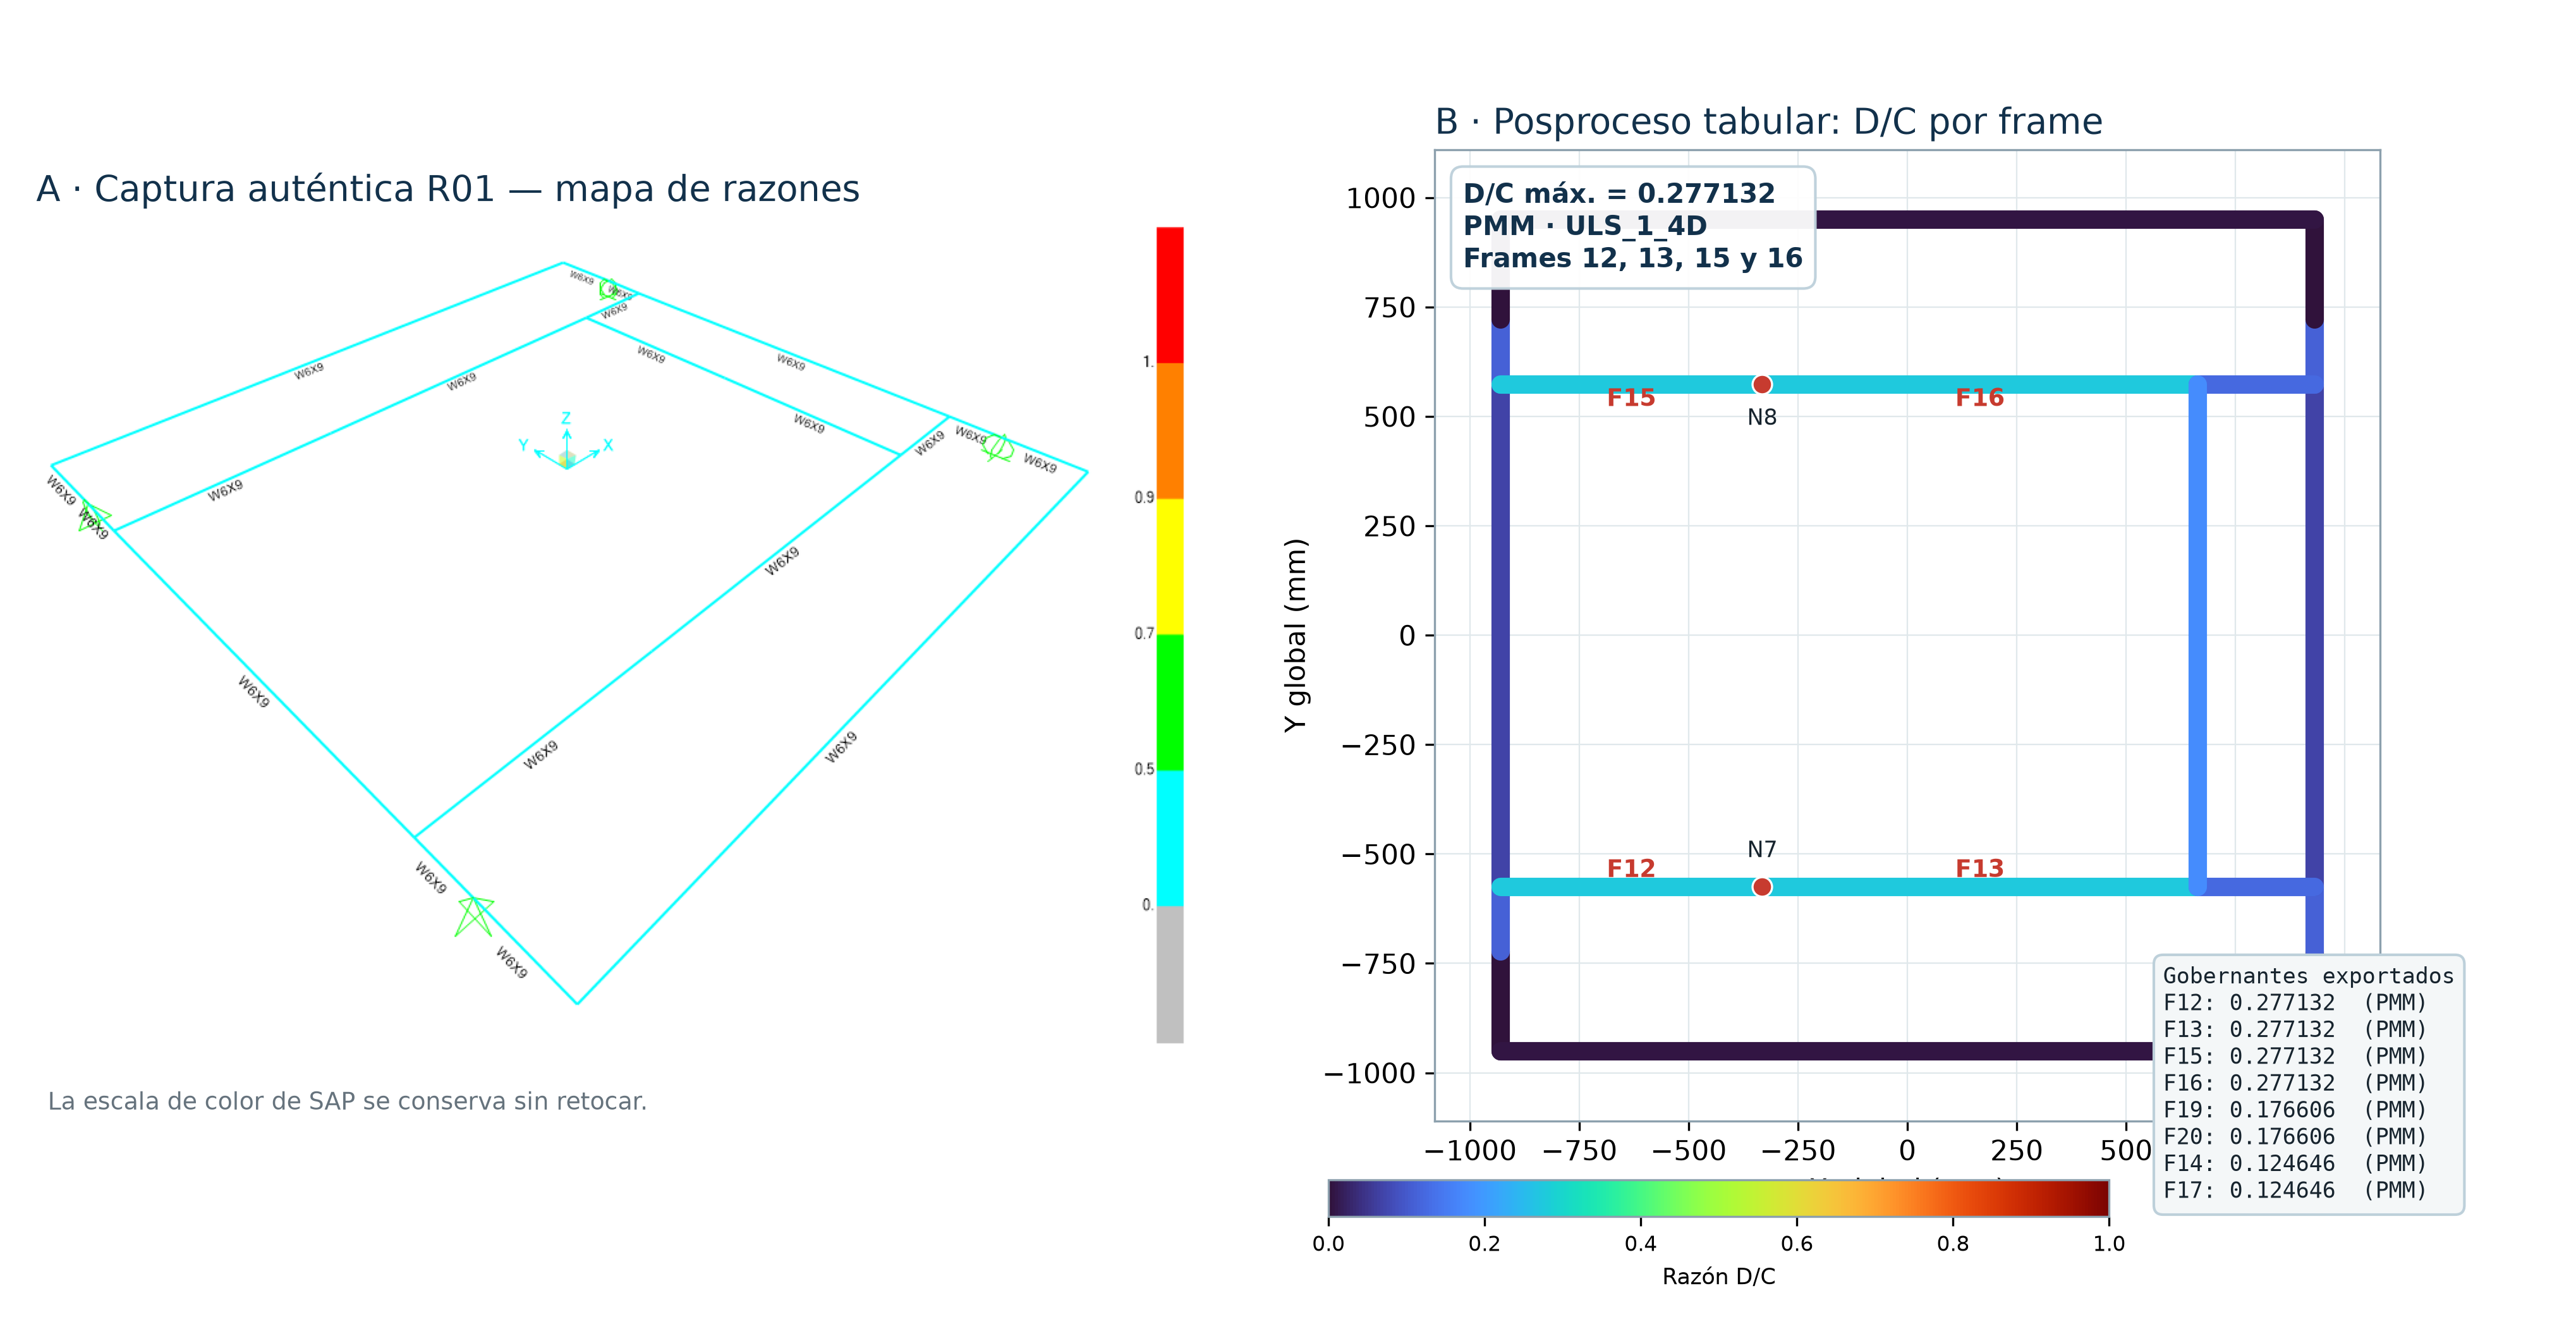
\includegraphics[width=\textwidth]{images/sap/04_VERIFICACION_RESISTENTE_R01_recorte.png}
\caption{Verificación resistente del bastidor con AISC 360-16 en SAP2000: razones demanda/capacidad por barra en la combinación ULS. Captura de la corrida de referencia.}
\label{fig:anx-resistencia-r01}
\end{figure}

\subsection{Respaldo del cálculo manual}
\label{sec:respaldo-complementario}

El caso manual de la Sección~\ref{sec:memoria-soporte} se contrasta con las hojas de coordenadas, cargas, reacciones y desplazamientos de \path{evidencias/N3_R01/R01_SAP_ORIGINAL.xlsx}. No se dispone del libro complementario \path{calculos/CALCULOS_SOPORTE_N3_N4_N5.xlsx}, citado como soporte de la hoja \emph{Contacto N3}; por ello, la extensión automática de ese desarrollo no forma parte de los entregables verificables. El libro mecánico de la revisión mecánica 5 contiene las hojas \emph{Ruedas}, \emph{PAD\_Contacto} y \emph{Auditoria\_R01}, pero responde a sus propios casos y no recalcula las corridas de cuatro y cinco apoyos.

\section{Libro mecánico de la revisión mecánica 5}
\label{sec:traza-ruedas-riel}

Las cargas de ruedas y riel de la Sección~\ref{sec:ruedas-rieles} se obtuvieron con el cálculo mecánico de esa revisión. La Tabla~\ref{tab:traza-ruedas-riel} relaciona cada magnitud con su hoja y celda en \path{evidencias/N3_R05/02_CALCULOS_EDITABLES_N3_R05.xlsx}. El procedimiento se desarrolla en \path{evidencias/N3_R05/01_CALCULO_R05_REPRODUCIBLE.py} y los resultados se almacenan en \path{evidencias/N3_R05/19_RESULTADOS_NUMERICOS_R05.json}. Este cálculo es independiente de la corrida estructural de referencia.

\begingroup
\small\singlespacing
\begin{longtable}{P{3.4cm}P{4.0cm}P{5.1cm}}
\caption{Trazabilidad de ruedas y riel en el libro mecánico de la revisión mecánica 5}\label{tab:traza-ruedas-riel}\\
\toprule
\textbf{Magnitud} & \textbf{Hoja y celda} & \textbf{Valor y alcance} \\
\midrule
Masa de cálculo & \texttt{Entradas!C7} & 3500 kg; escenario de diseño \\
Masa estimada & \texttt{Masa\_CG!B20} & 3439,831288 kg; balance de masas \\
Peso de cálculo & \texttt{Ruedas!B19} & 34,335 kN \\
Carga de servicio & \texttt{Ruedas!B7} & 21,865488 kN; factor 1,15 \\
Carga resistente local & \texttt{Ruedas!B8} & 26,618855 kN; factor 1,40 \\
Reacción de instalación & \makecell[l]{\texttt{Riel\_Envolvente}\\\texttt{B13}} & 26,741372 kN; apoyo del riel \\
Momento del vano simple & \makecell[l]{\texttt{Riel\_Envolvente}\\\texttt{B16}} & 3956529,787 N\,mm; carga resistente \\
Esfuerzos de cabeza y base & \makecell[l]{\texttt{Riel\_Envolvente}\\\texttt{B17:B18}} & 146,538140 y 95,338067 MPa \\
Flecha de servicio & \makecell[l]{\texttt{Riel\_Envolvente}\\\texttt{B19}} & 0,531864 mm; carga de servicio \\
\bottomrule
\end{longtable}
\endgroup

El caso manual se identifica como \texttt{3C\_W1\_MP} en el código y en \texttt{wheel\_cases} del archivo de resultados. El libro identifica primero el caso simétrico \texttt{3C-03}, con la rueda 3 ausente y $e_x=e_y=+100$ mm; ambos alcanzan el mismo máximo sin factor, de 19,013468 kN. Las funciones \texttt{wheel\_cases} y \texttt{rail\_envelope} contienen los barridos restantes. El bloque \texttt{rail.governing\_continuous} localiza la reacción de instalación en el riel derecho, apoyo 2, caso \texttt{3C\_W4\_PM}, con el centro de la mesa en $Y=-3320{,}038$ mm y una carga de rueda de 26,618855 kN en $Y=-4042{,}038$ mm. El mínimo de la sensibilidad continua, $-3{,}691891$ kN, corresponde a los apoyos riel--base y no al contacto rueda--riel; esa sensibilidad usa restricciones bilaterales y no valida la retención ni el diseño civil.

La configuración vigente, con doce apoyos por riel, se recalculó en la revisión de integración (\path{estructural/integracion_R06/00_ANALISIS_PREVIOS_2026-09-24/J2_soportes_riel_recalculo.md}): reacción máxima de apoyo de 26,623 kN y mínima de $-3{,}779$ kN en ULS, esfuerzos de cabeza y base de 97,92 y 63,71 MPa y flechas entre apoyos de 0,260 mm en servicio y 0,317 mm en ULS, valores resumidos en la Tabla~\ref{tab:ruedas-rieles}.

\section{Modelo de mojado: configuración y verificación}
\label{sec:anx-cfd}

La Tabla~\ref{tab:anx-cfd-config} reúne la configuración del modelo de mojado de la Sección~\ref{sec:resultados-aspersion}. Los journals, las tablas de inyección, las transcripciones y los resultados se conservan en \path{cfd/02_configuracion_base_22/} y \path{cfd/03_configuracion_propuesta_24/}; los casos de Fluent y los impactos exportados no se publican por su tamaño. Los guiones \path{rayos_r05.py}, \path{post_kpi.py}, \path{combinar_kpi.py}, \path{tabla_k1k6.py} y \path{balance_global_22.py} calculan las máscaras de sombra, los indicadores y el balance. Un recálculo independiente de los indicadores de dosis, uniformidad, zona seca, transferencia e impulso a partir de los impactos reprodujo los valores con diferencias menores que 1\,\%; las máscaras y el acceso geométrico se reprodujeron exactamente al ejecutar de nuevo el mismo trazado de rayos, lo que confirma su reproducibilidad, pero no es un método independiente.

\begingroup
\small\singlespacing
\setlength{\tabcolsep}{4pt}
\begin{longtable}{@{}>{\raggedright\arraybackslash}p{3.4cm}>{\raggedright\arraybackslash}p{\dimexpr\textwidth-3.4cm-4\tabcolsep\relax}@{}}
\caption{Configuración del modelo de mojado}\label{tab:anx-cfd-config}\\
\toprule
\textbf{Aspecto} & \textbf{Configuración}\\
\midrule\endfirsthead
\toprule
\textbf{Aspecto} & \textbf{Configuración}\\
\midrule\endhead
\bottomrule\endlastfoot
Programa & ANSYS Fluent 2026 R1, versión estudiantil, limitada a 1\,048\,576 celdas\\
Régimen & Transitorio; $\Delta t=5\times10^{-5}$ s con 10 iteraciones por paso\\
Fase continua & Aire con turbulencia $k$--$\varepsilon$ estándar a 76,24 kPa (escenario de 2335 m)\\
Fase discreta & Lagrangiana, acoplada en dos vías, sin dispersión turbulenta estocástica; líquido de 982,12 kg/m$^3$ a 62~$^\circ$C\\
Inyección & Abanico de 50$^\circ$ con 2$^\circ$ de espesor; gotas con distribución de Rosin--Rammler de diámetro característico 300 µm y exponente 2,5, supuesta; velocidad de salida $0{,}95\sqrt{2p/\rho}$, de unos 27,5 m/s; caudal y presión de cada boquilla según la red de 22 boquillas; 600 trayectorias por plano y tres planos de espesor (1200 en las boquillas inferiores). En la configuración propuesta, las cuatro boquillas inferiores tienen un abanico de 15$^\circ$, interpolado a 16,8$^\circ$ a 4 bar (hipótesis), y los caudales de la red de 24 boquillas\\
Paredes y fronteras & Retención de la gota en el primer impacto; fronteras abiertas a la presión del sitio\\
Dominios & Sector de las boquillas laterales e inferior exterior del brazo exterior A (430\,560 celdas) y el mismo sector para el brazo B; sector de 90$^\circ$ para la boquilla inferior de la lanza (197\,280); sector de la cara superior (237\,552); dominio polar completo del agujero (512\,130)\\
Malla & Hexaédrica estructurada; tamaño máximo de 4 mm en dirección radial, 0,5$^\circ$ en la angular y 5 mm en la axial\\
Movimiento del aplicador & Detenido; dosis por vuelta a 1,7 rpm integrando la huella sobre la circunferencia\\
Obstáculos & Apoyos sectoriales, topes y vigas como máscaras de sombra por trazado de rayos, con la geometría del soporte\\
Posproceso & Indicadores por bandas de 10 mm (definición principal) y de 2 mm (complementaria)\\
\end{longtable}
\endgroup

La Figura~\ref{fig:anx-dominio} muestra el dominio sectorial de $\pm12^\circ$ y la malla hexaédrica del sector de las boquillas laterales y de la inferior exterior, con sus fronteras abiertas. La Figura~\ref{fig:anx-aire} ilustra el efecto que incorpora el acoplamiento en dos vías: el chorro arrastra el aire hacia la pared, y ese aire frena las gotas de la parte baja del diámetro exterior.

\begin{figure}[htbp]
\centering
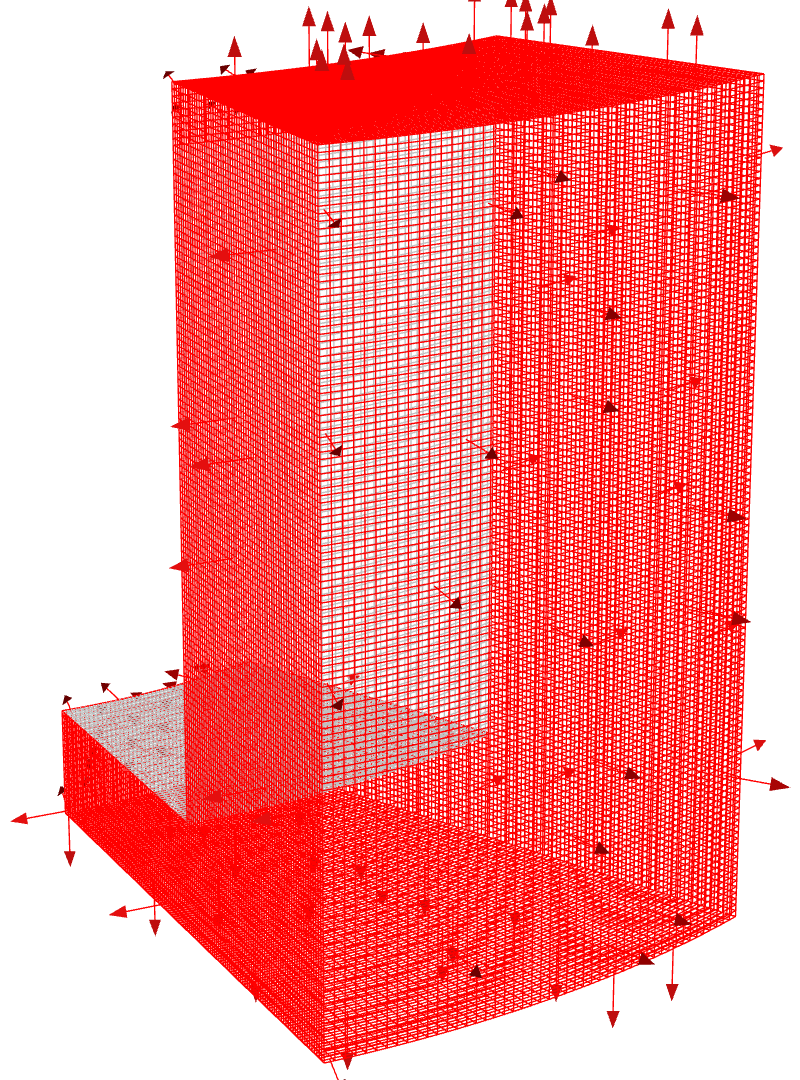
\includegraphics[width=0.55\textwidth]{fluent_dominio_malla_od.png}
\caption[Dominio y malla del sector de las boquillas laterales e inferior exterior]{Dominio de cálculo y malla hexaédrica del sector de $\pm12^\circ$ de las boquillas laterales y de la inferior exterior de un brazo (diámetro exterior y cara inferior), vista isométrica; las flechas señalan las fronteras abiertas. Elaboración propia, ANSYS Fluent 2026 R1 (licencia Student); imagen recortada al área de interés.}
\label{fig:anx-dominio}
\end{figure}

\begin{figure}[htbp]
\centering
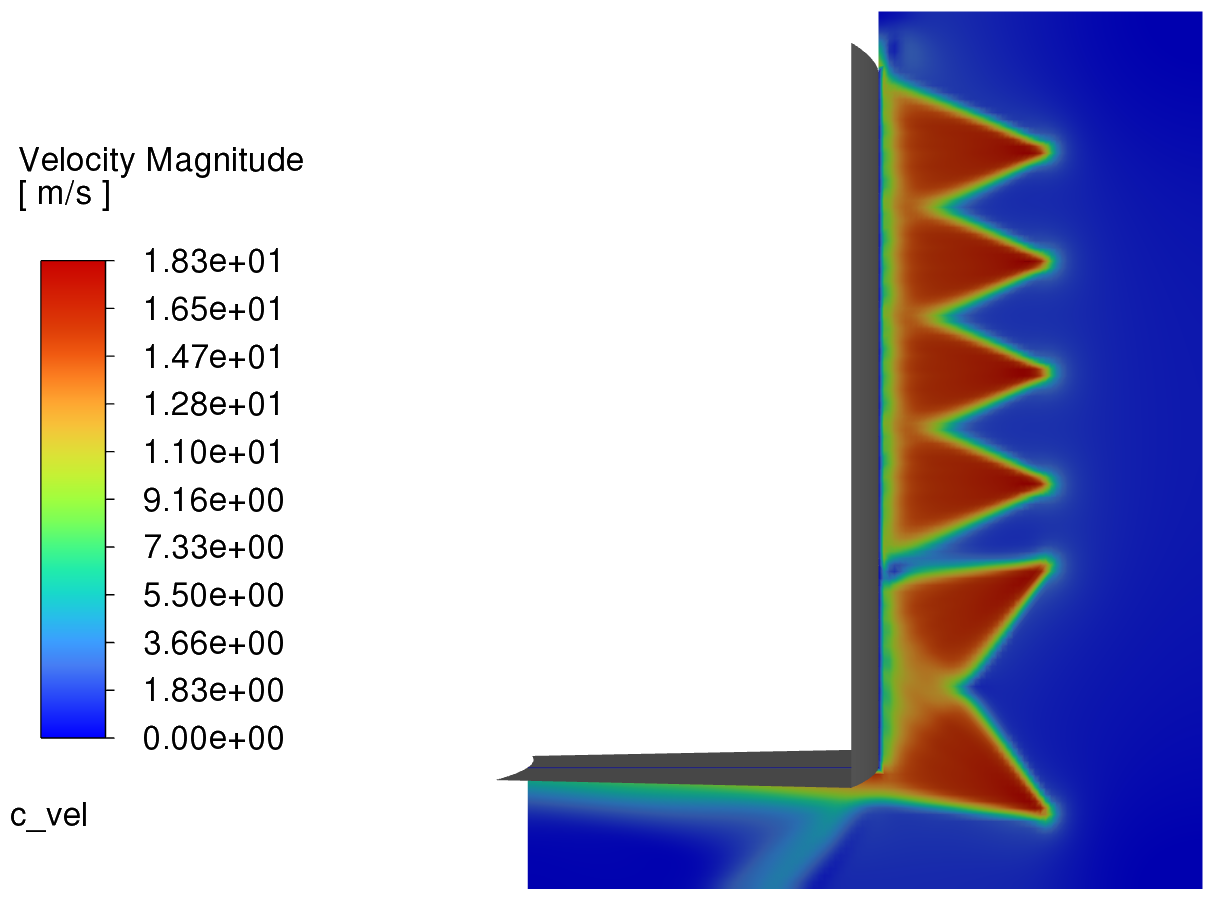
\includegraphics[width=0.70\textwidth]{fluent_aire_arrastrado_od.png}
\caption[Velocidad del aire arrastrado por los chorros]{Velocidad del aire en el plano de los abanicos de las boquillas laterales y de la inferior exterior de un brazo, configuración base. Es un campo de la fase continua, no un indicador. La escala de color es la magnitud de la velocidad en m/s (rótulo del programa en inglés). Elaboración propia, simulación en ANSYS Fluent 2026 R1 (licencia Student); imagen recortada al área de interés.}
\label{fig:anx-aire}
\end{figure}

La velocidad de salida se calculó con un coeficiente de 0,95 sobre la velocidad ideal, lo que da 27,11--27,59 m/s. Como contraste, la continuidad con el orificio equivalente de catálogo, de 0,109 pulgadas (2,77 mm), y el caudal de cada toma da 25,24--25,68 m/s, un 7\,\% menos; ese orificio implica un coeficiente de descarga de 0,884 (Sección~\ref{sec:man-asp-boquilla}). El modelo de mojado registró velocidades normales de impacto de 23,0 a 23,4 m/s en el diámetro exterior, la cara superior y el agujero, por debajo de ambas estimaciones, como corresponde al frenado aerodinámico de las gotas en los 126 a 185 mm de vuelo. Como el impulso es proporcional a la velocidad de las gotas a igual caudal, adoptar la velocidad por continuidad reduciría $\bar J$ en un 7\,\% como máximo; la dosis y la transferencia dependen sobre todo del caudal, que es el mismo en ambos casos.

La Tabla~\ref{tab:verificacion-cfd} reúne los cambios de los indicadores entre las dos mallas más finas, con el paso de tiempo a la mitad y con el dominio ampliado.

\begin{table}[htbp]
\centering\small\singlespacing
\caption{Verificación numérica del modelo de mojado: cambio respecto de la corrida base}
\label{tab:verificacion-cfd}
\begin{tabular}{lcccc}
\toprule
\textbf{Estudio} & \textbf{$\bar D$} & \textbf{CV (absoluto)} & \textbf{$\bar J$} & \textbf{$\eta$}\\
\midrule
Malla fina, cara superior & $-0{,}08$\,\% & $-0{,}0039$ & $+0{,}54$\,\% & $-0{,}07$\,\%\\
Malla fina, diámetro exterior & $-0{,}11$\,\% & $-0{,}0002$ & $+0{,}75$\,\% & $-0{,}12$\,\%\\
Malla fina, cara inferior (exterior) & $+0{,}61$\,\% & $-0{,}0151$ & $+1{,}01$\,\% & $+0{,}57$\,\%\\
Malla fina, cara inferior (lanza) & $-0{,}19$\,\% & $+0{,}0012$ & $+0{,}30$\,\% & $-0{,}18$\,\%\\
Paso de tiempo a la mitad & $\leq0{,}01$\,\% & $\leq0{,}0001$ & $\leq0{,}04$\,\% & $\leq0{,}02$\,\%\\
Dominio ampliado & $\leq0{,}14$\,\% & $\leq0{,}0084$ & $\leq0{,}27$\,\% & $\leq0{,}02$\,\%\\
\bottomrule
\end{tabular}
\par\smallskip\footnotesize
$\bar D$: dosis media; CV: coeficiente de variación; $\bar J$: impulso medio; $\eta$: transferencia.
\end{table}

La Tabla~\ref{tab:anx-gci} contiene el estudio de malla de tres niveles de la configuración base y la Figura~\ref{fig:anx-verificacion-cfd}, la dosis media y la presión de huella de cada malla normalizadas con las de la malla fina. Cuando el cambio entre las dos mallas finas es menor que el ruido entre corridas equivalentes de los brazos exteriores A y B, el índice de convergencia de malla no es interpretable y basta con comprobar que el cambio sea pequeño.

\begin{table}[htbp]
\centering\small\singlespacing
\setlength{\tabcolsep}{2.5pt}
\caption{Estudio de malla del modelo de mojado: índice de convergencia de la malla fina}
\label{tab:anx-gci}
\begin{tabular}{lcccccc}
\toprule
\textbf{Dominio} & \textbf{Celdas (miles)} & \textbf{$r_{21}$; $r_{32}$} & \textbf{$\bar D$} & \textbf{CV} & \textbf{$\bar J$} & \textbf{$\eta$}\\
\midrule
Cara superior & 112 / 238 / 465 & 1,251; 1,283 & 0,07\,\% & 2,20\,\% & 1,47\,\% & 0,05\,\%\\
Diámetro exterior & 203 / 431 / 847 & 1,253; 1,286 & 0,30\,\% & 0,68\,\% & 4,45\,\% & 0,25\,\%\\
Cara inferior, exterior* & 203 / 431 / 847 & 1,253; 1,286 & 3,92\,\% & 12,55\,\% & 4,88\,\% & 5,82\,\%\\
Cara inferior, lanza & 91 / 197 / 381 & 1,246; 1,295 & 0,18\,\% & 0,06\,\% & 1,44\,\% & 0,17\,\%\\
Borde del agujero, lanza & 91 / 197 / 381 & 1,246; 1,295 & 0,11\,\% & 1,07\,\% & 1,62\,\% & 0,14\,\%\\
\bottomrule
\end{tabular}
\par\smallskip\footnotesize
*Cambios entre mallas dentro del ruido entre los brazos A y B: índice no interpretable. Procedimiento de \cite{celik2008}.
\end{table}

\begin{figure}[htbp]
\centering
\begin{minipage}[t]{0.49\textwidth}\centering
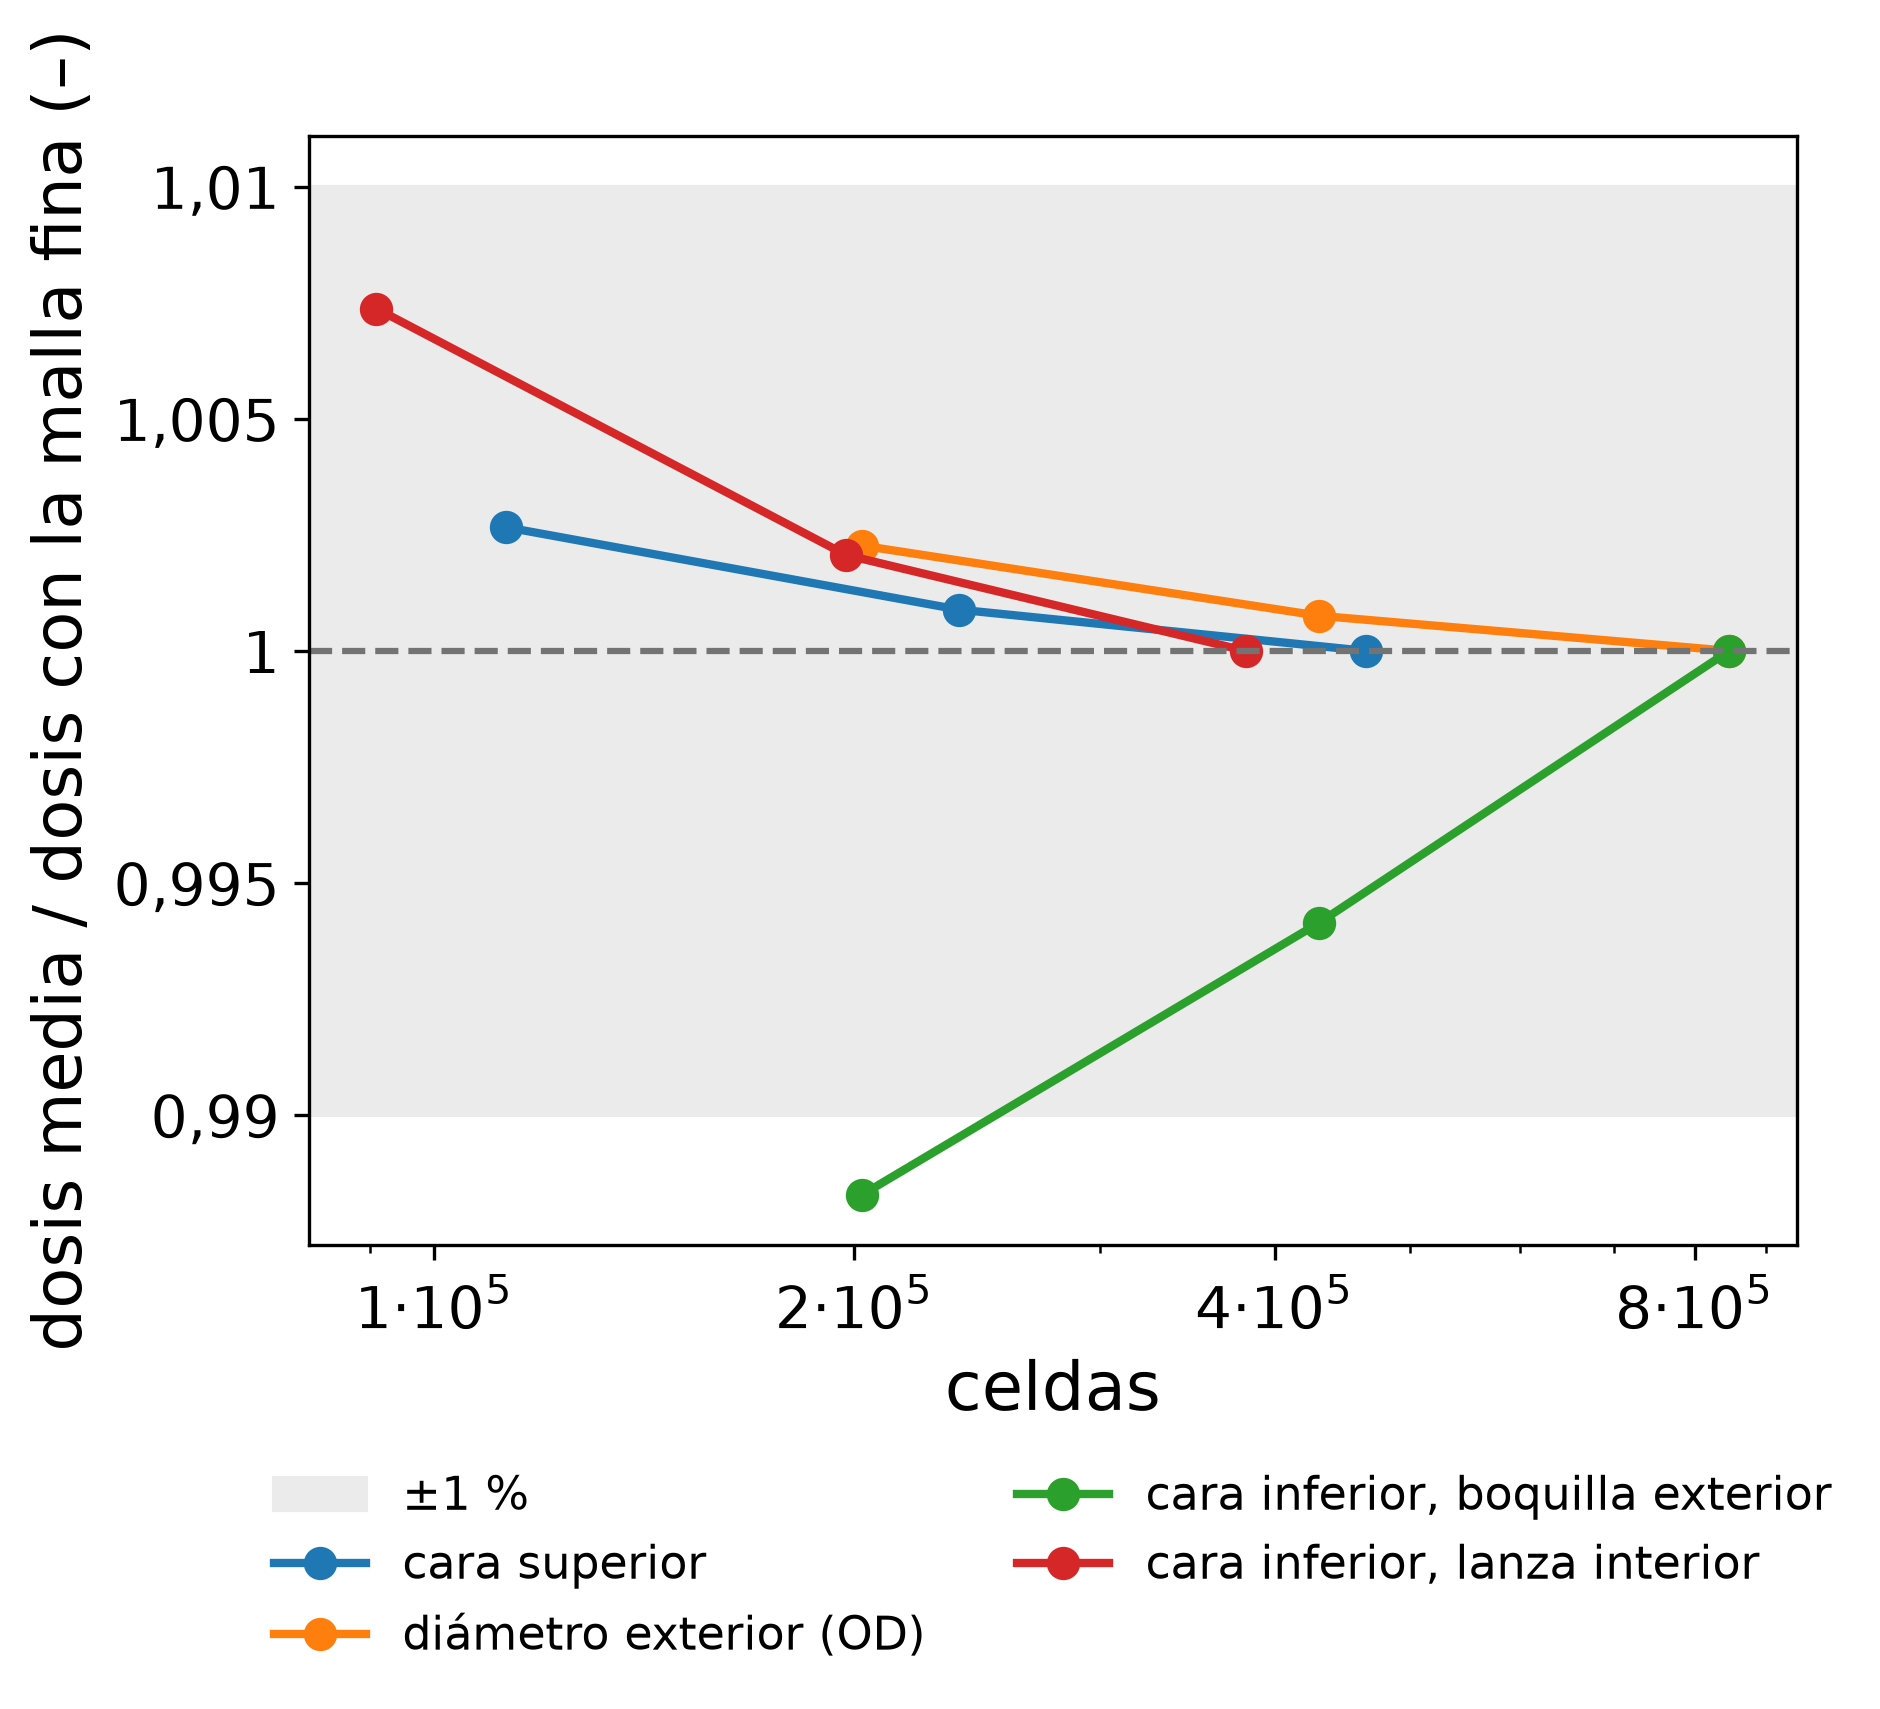
\includegraphics[width=\linewidth]{F11_DPM_dosis_media_frente_a_malla.png}\par\small (a)
\end{minipage}\hfill
\begin{minipage}[t]{0.49\textwidth}\centering
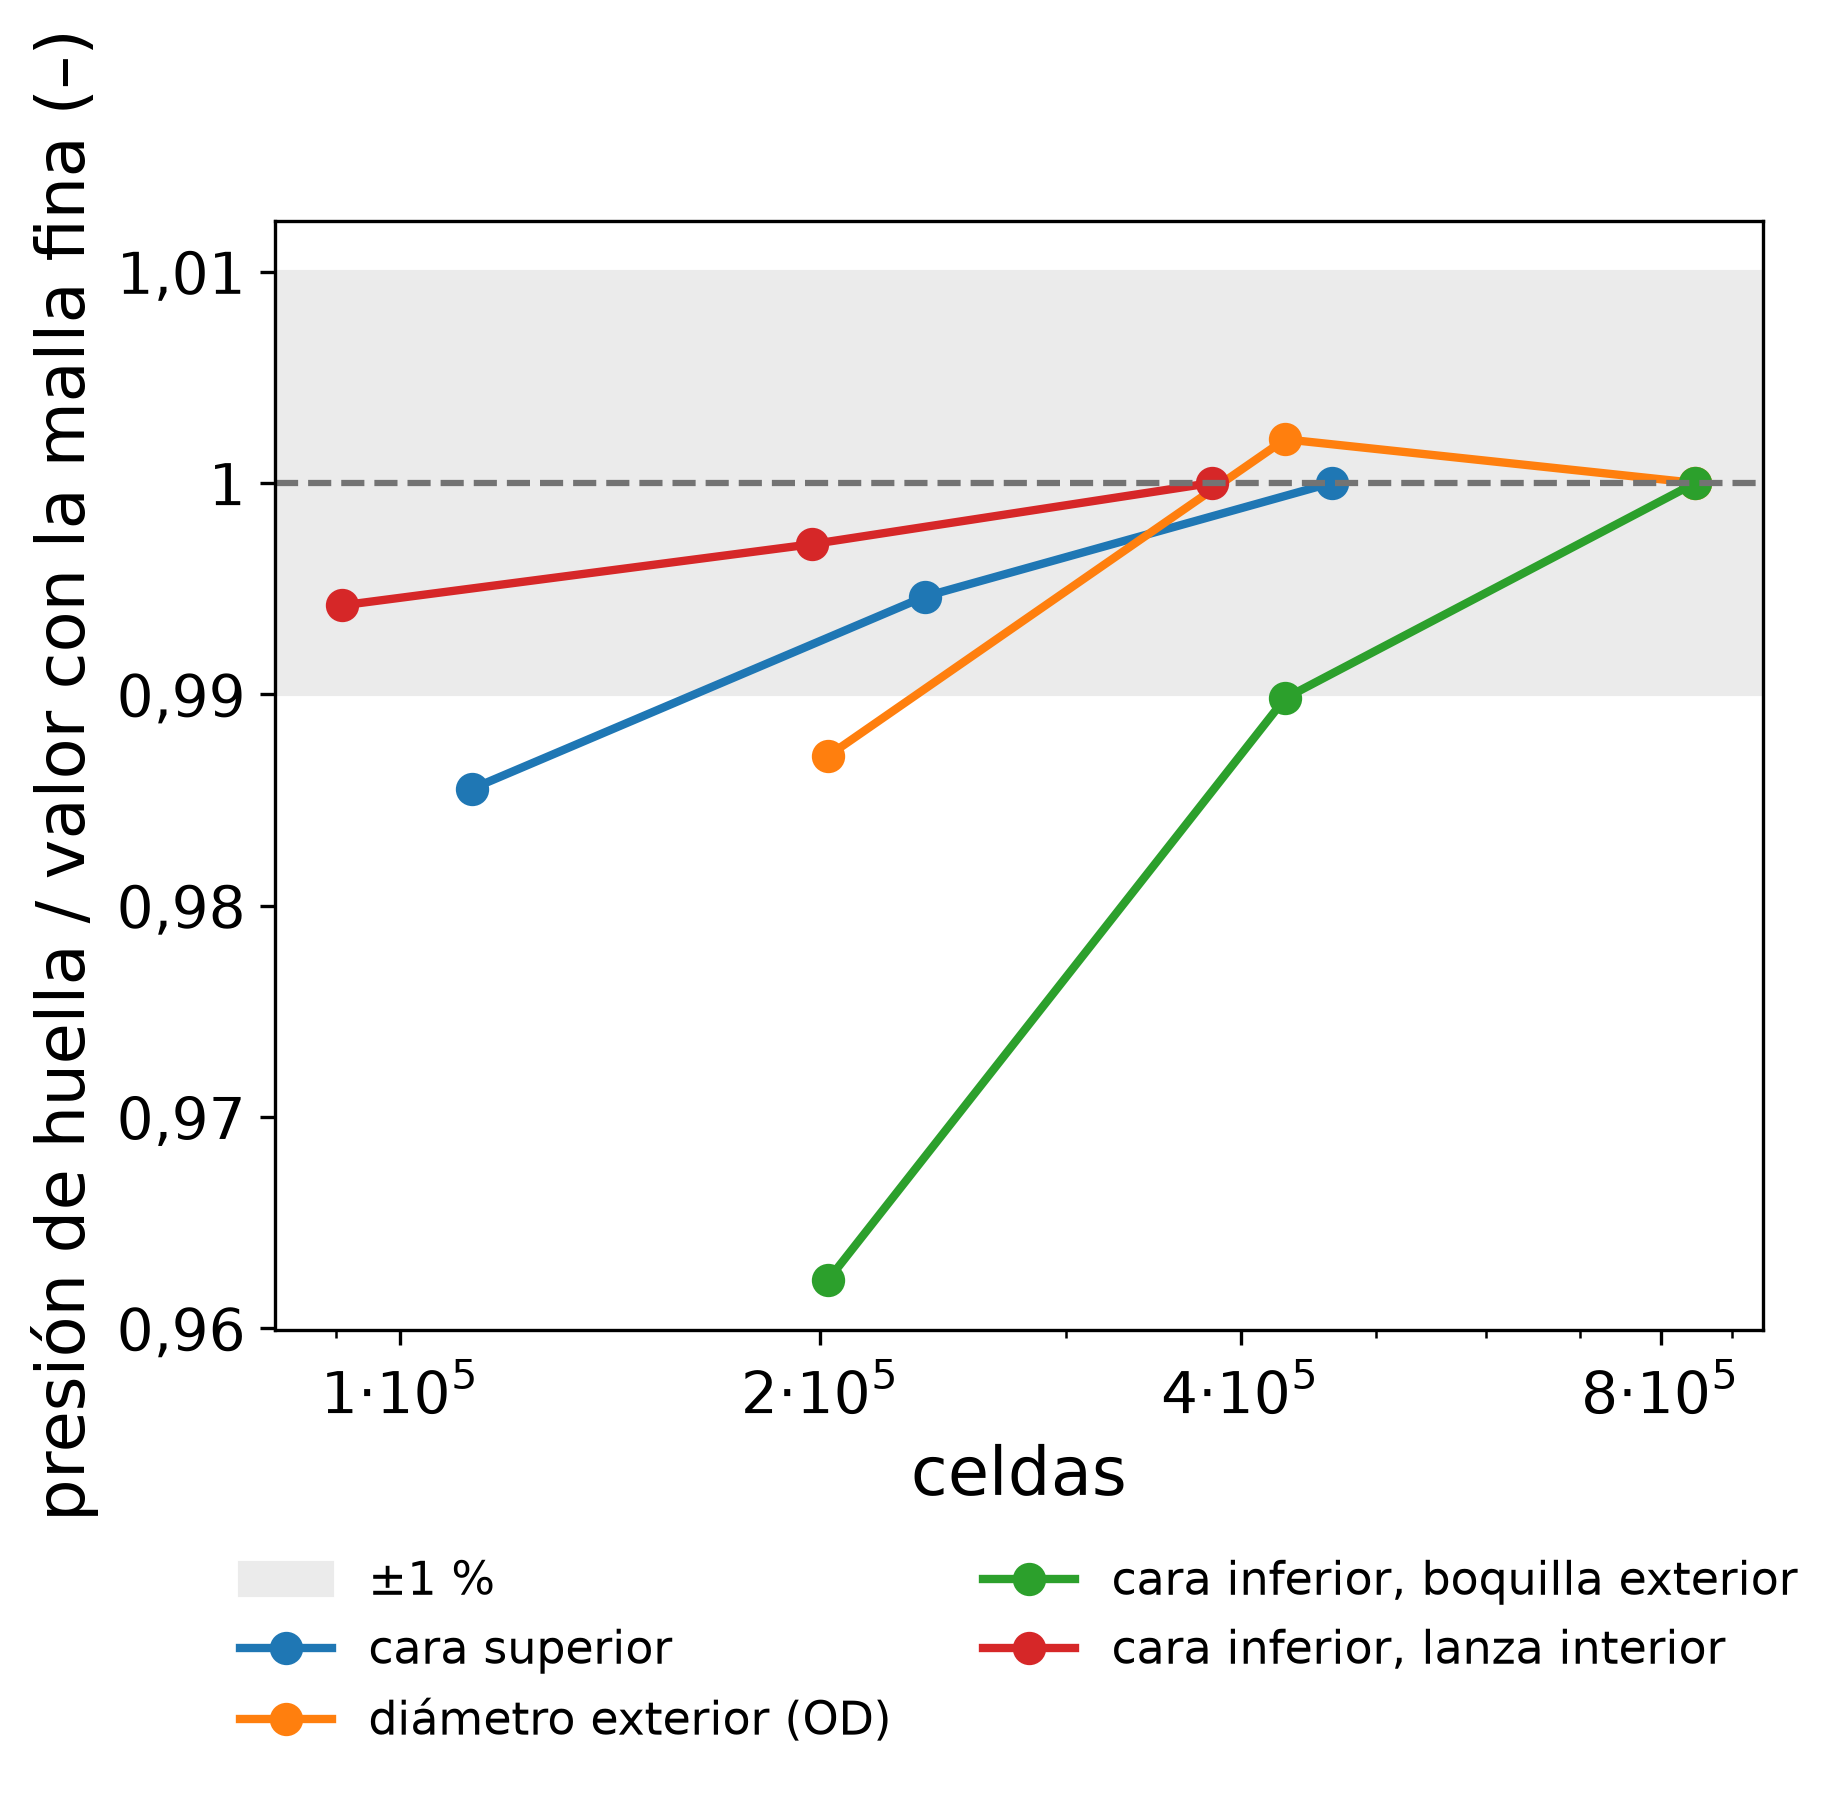
\includegraphics[width=\linewidth]{F12_DPM_presion_huella_frente_a_malla.png}\par\small (b)
\end{minipage}
\caption[Verificación de malla del modelo de mojado de la configuración base]{Verificación de malla de la configuración base: (a) dosis media y (b) presión de huella de cada malla, normalizadas con las de la malla fina. Verificación numérica, no validación. Elaboración propia con los resultados de ANSYS Fluent.}
\label{fig:anx-verificacion-cfd}
\end{figure}

En esa configuración el paso de tiempo fue fijo, de modo que el número de Courant de las gotas creció con el refinamiento: 0,27, 0,34 y 0,43 en las tres mallas. Para descartar que ese crecimiento afectara el estudio, las mallas gruesa y fina de los tres dominios se repitieron con el paso de tiempo ajustado para mantener el Courant de gota en 0,34 (0,27 en la cara superior). Los cambios entre las dos mallas más finas fueron los mismos que con el paso fijo: las diferencias entre ambas series no pasaron de 0,03 puntos porcentuales en la dosis media ni de 0,07 en el impulso medio, y los balances de masa quedaron entre 0,02 y 0,14\,\%. En la configuración propuesta se ajustó el paso de tiempo de cada malla para mantenerlo cerca de 0,339 desde el principio (Sección~\ref{sec:resultados-aspersion}).

La Tabla~\ref{tab:anx-mascaras} compara el método de máscaras con una corrida en la que un apoyo sectorial se incluyó en la malla, y la Tabla~\ref{tab:anx-puente} resume el caso puente entre OpenFOAM y Fluent en el agujero.

\begin{table}[htbp]
\centering\small\singlespacing
\caption{Sombras por trazado de rayos frente a un apoyo incluido en la malla: fracción del caudal de la boquilla que llega a cada destino}
\label{tab:anx-mascaras}
\begin{tabularx}{\textwidth}{@{}YP{2.6cm}P{3.4cm}@{}}
\toprule
\textbf{Boquilla y destino} & \textbf{Trazado de rayos (\%)} & \textbf{CFD con el apoyo en la malla (\%)}\\
\midrule
Inferior exterior $\rightarrow$ apoyos sectoriales & 18,0 & 16,9\\
Inferior exterior $\rightarrow$ cara inferior, sin apoyos & 20,7 & 21,0\\
Inferior exterior $\rightarrow$ cara inferior, con apoyos & 4,0 & 4,5\\
Lateral 5 $\rightarrow$ apoyos sectoriales & 12,7 & 9,2\\
\bottomrule
\end{tabularx}
\par\smallskip\footnotesize
Configuración base. Verificación del método, no validación.
\end{table}

\begin{table}[htbp]
\centering\small\singlespacing
\caption{Caso puente del agujero: OpenFOAM frente a ANSYS Fluent}
\label{tab:anx-puente}
\begin{tabular}{@{}>{\raggedright\arraybackslash}p{4.6cm}cccc@{}}
\toprule
\textbf{Indicador} & \textbf{OpenFOAM} & \textbf{Fluent} & \textbf{Diferencia} & \textbf{Criterio}\\
\midrule
Caudal depositado (kg/s) & 0,7835 & 0,7814 & $-0{,}26$\,\% & ---\\
Dosis media (kg\,m$^{-2}$ por vuelta) & 18,809 & 18,759 & $-0{,}27$\,\% & $\leq5$\,\%\\
Coeficiente de variación & 0,3397 & 0,3362 & $-0{,}0035$ & $\leq0{,}03$\\
Zona seca (\%) & 0 & 0 & 0 & 0 en ambos\\
Curvas de cobertura, diferencia máxima & --- & --- & 1,33 puntos & $\leq2$ puntos\\
\bottomrule
\end{tabular}
\end{table}

\begin{figure}[htbp]
\centering
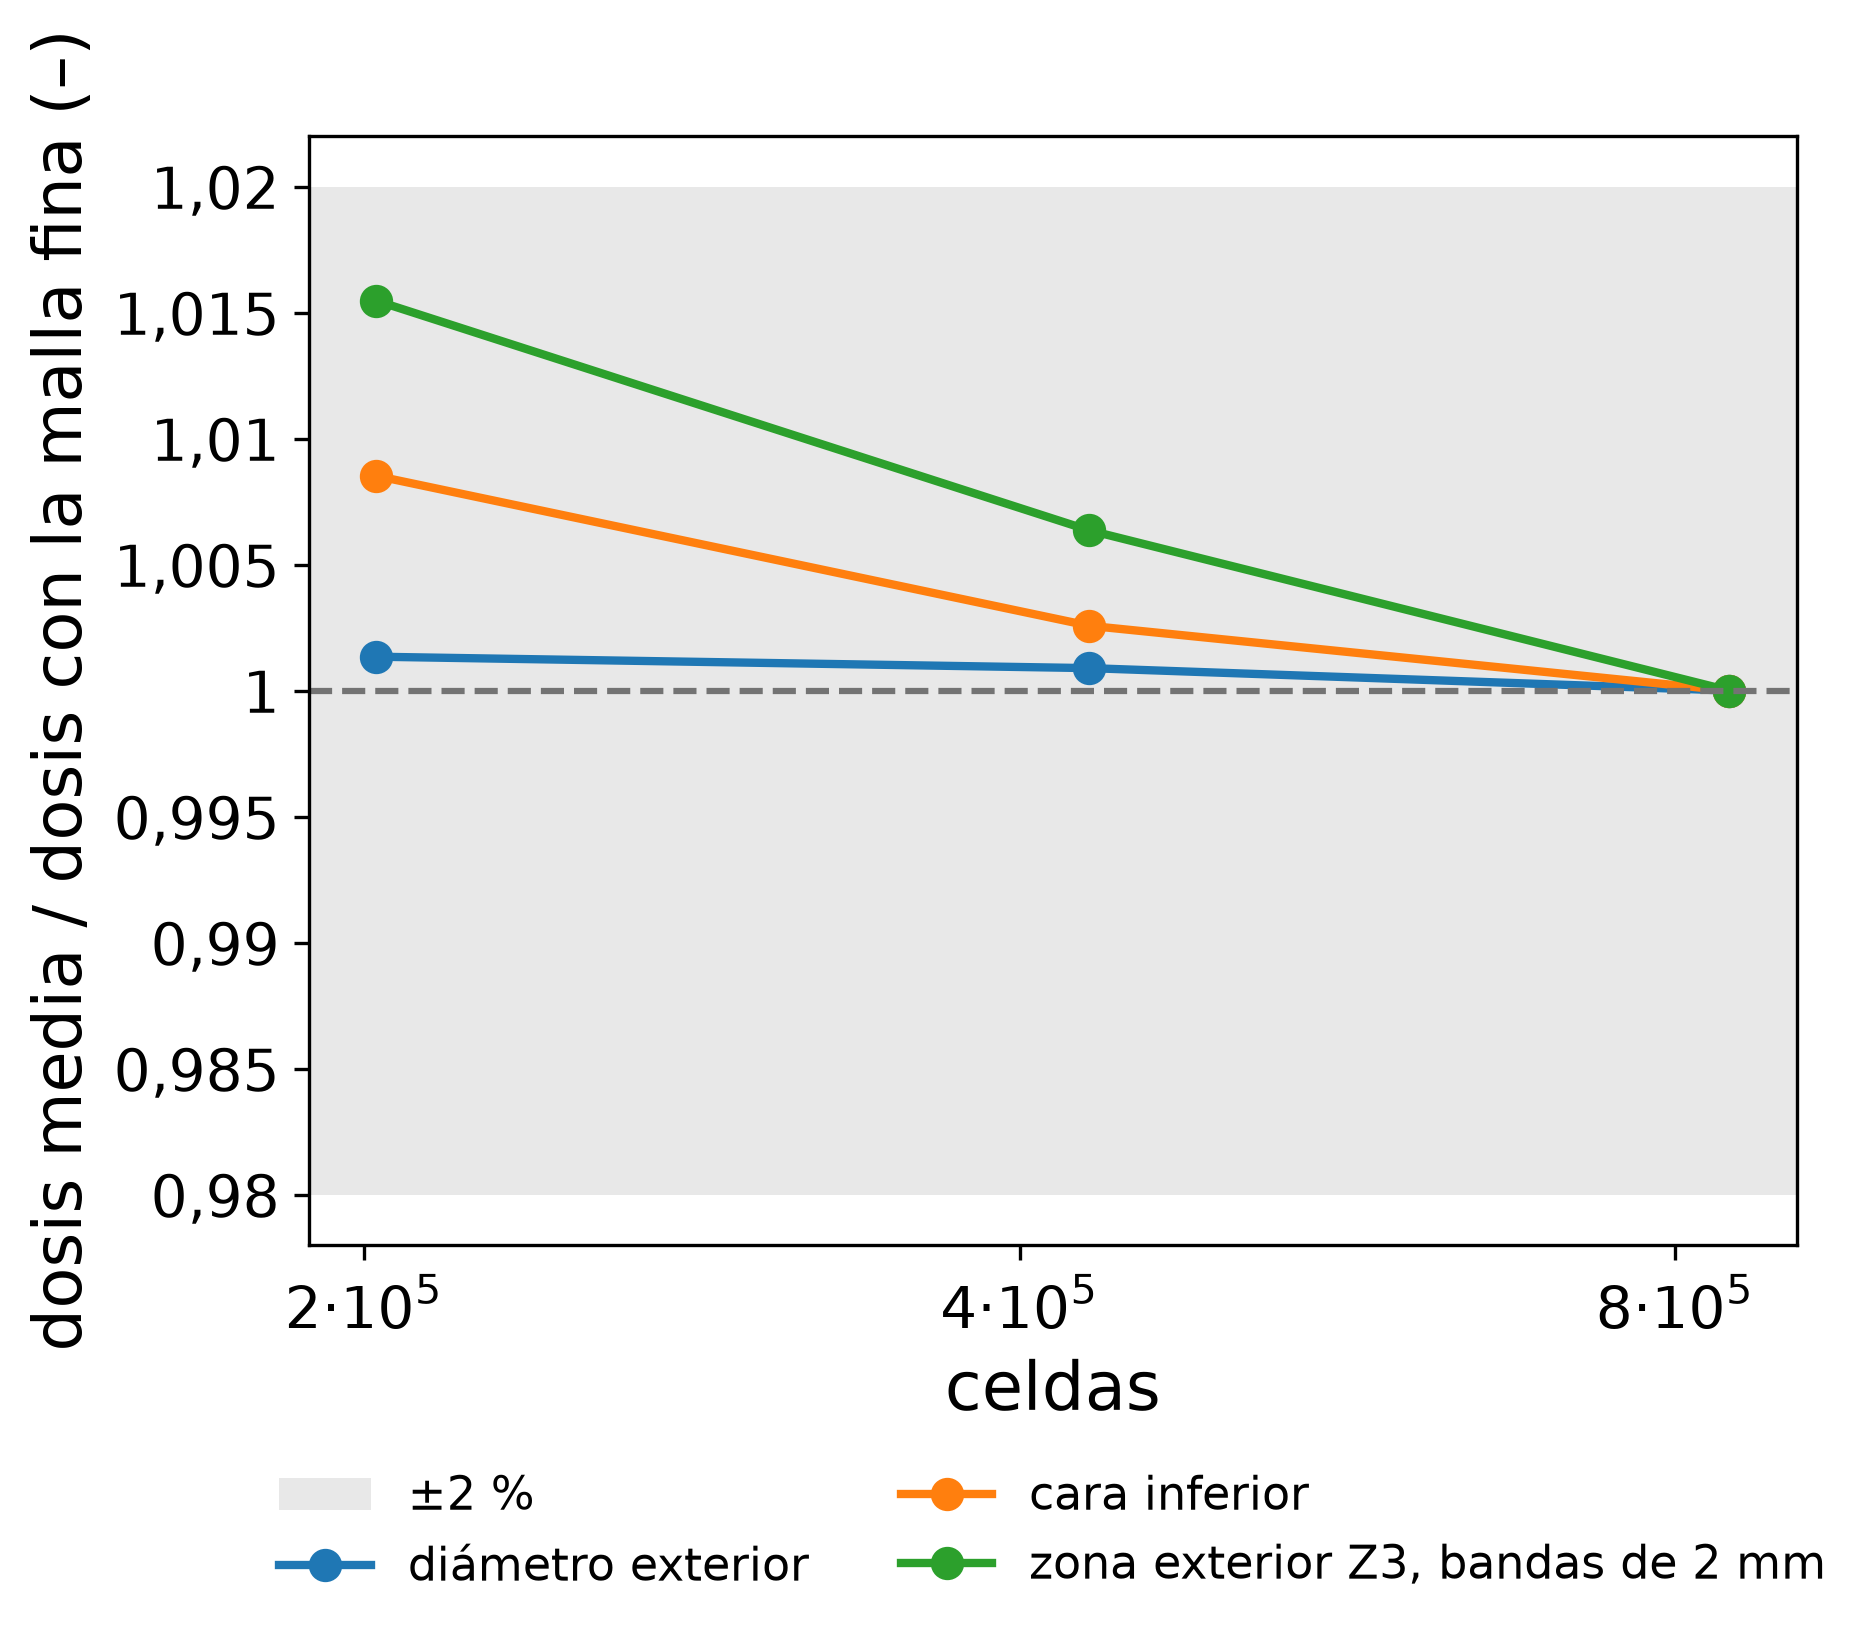
\includegraphics[width=0.55\textwidth]{fig_malla_configuracion_propuesta.png}
\caption{Dosis media de la configuración propuesta de 24 boquillas con tres mallas, normalizada con la de la malla fina. Elaboración propia con los datos exportados de ANSYS Fluent.}
\label{fig:cfd-malla-propuesta}
\end{figure}

\section{Tiempo de lavado y sombras de la cara inferior}
\label{sec:anx-tiempo-lavado}

La dosis acumulada después de $N$ vueltas en una banda o en una celda es $N\,D$, con $D$ la dosis por vuelta de la Ecuación~\eqref{eq:teo-dosis}. El tiempo $t_{95}$ de la Tabla~\ref{tab:tiempo-lavado} es el menor número entero de vueltas para el que el 95\,\% del área accesible cumple $N\,D\geq D_{req}$, multiplicado por los 35,3 s de una vuelta. La lectura por bandas usa la dosis media de cada anillo de 10 mm. La lectura por celdas usa el mapa de 10 mm por 0,5$^\circ$ exportado del CFD con las máscaras de sombra, que distingue las zonas donde un apoyo o un tope tapa solo una parte de los chorros durante la vuelta.

\begin{table}[htbp]
\centering\small\singlespacing
\caption{Tiempo para que el 95\,\% del área accesible alcance la dosis requerida}
\label{tab:tiempo-lavado}
\begin{tabular}{@{}llccc@{}}
\toprule
\textbf{Superficie} & \textbf{Lectura} & \textbf{65 kg\,m$^{-2}$} & \textbf{183 kg\,m$^{-2}$} & \textbf{305 kg\,m$^{-2}$}\\
\midrule
Diámetro exterior & Bandas y celdas & 2,9 & 8,2 & 14,1\\
Cara superior & Bandas y celdas & 4,1 & 10,6 & 17,6\\
Agujero & Bandas y celdas & 2,9 & 8,2 & 14,1\\
Cara inferior & Bandas de 10 mm & 5,3 & 14,1 & 23,5\\
 & Celdas de 10 mm $\times$ 0,5$^\circ$ & 27,1 & 75,9 & $>120$\\
\bottomrule
\end{tabular}
\par\smallskip\footnotesize
Tiempos en minutos, en vueltas enteras de 35,3 s a 1,7 rpm y con un horizonte de 120 min; 24 boquillas, con la boquilla superior en su posición base. Las bandas toman la dosis media de cada anillo de 10 mm; las celdas resuelven además la posición angular y registran las sombras parciales de las bases de los apoyos sectoriales y de los topes.
\end{table}

En el diámetro exterior, la cara superior y el agujero no hay sombras parciales, y las dos lecturas coinciden. En la cara inferior, el 10,4\,\% del área accesible tiene un factor de sombra menor que 0,25 y el 3,2\,\%, entre 0,25 y 0,5; corresponden a las bases de los apoyos sectoriales y a los topes de retención. Por eso la curva por celdas de la Figura~\ref{fig:anx-tiempo-lavado} sube rápido hasta un 83\,\% del área y después avanza despacio: el último 12\,\% es la zona sombreada.

\begin{figure}[htbp]
\centering
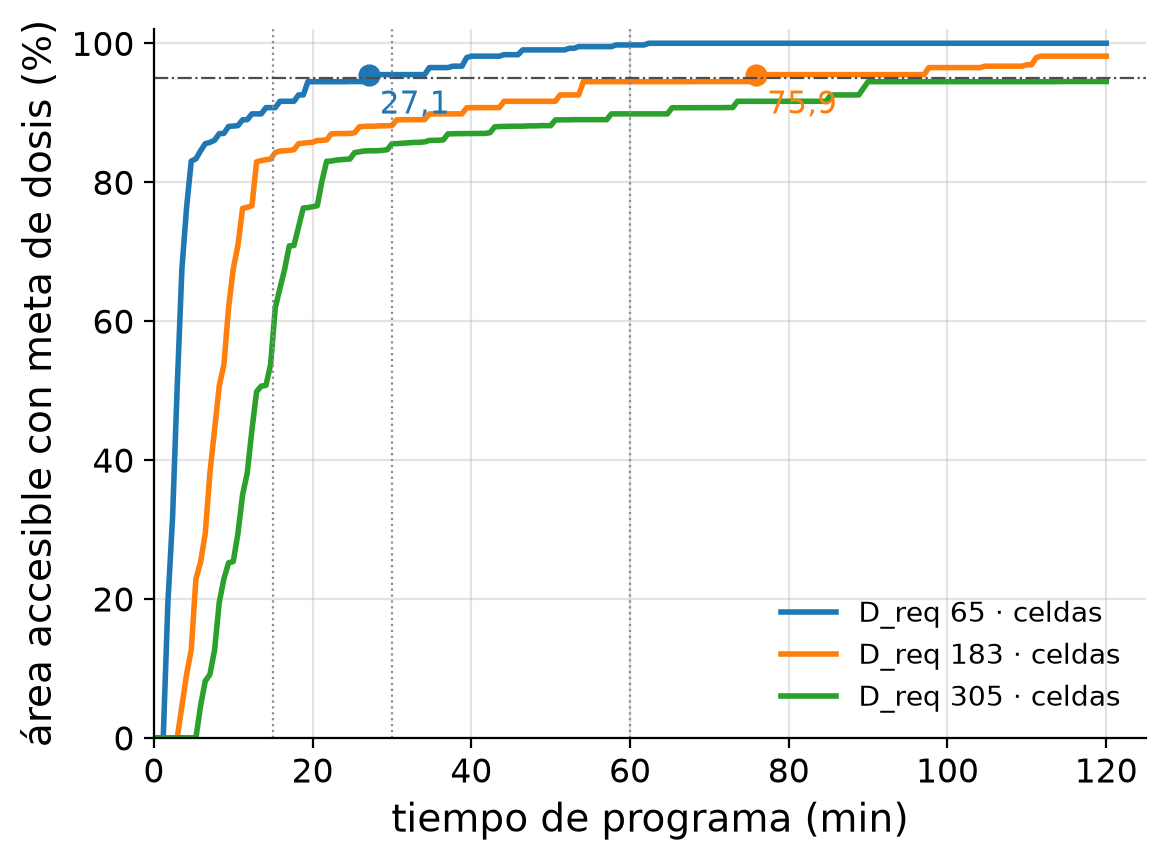
\includegraphics[width=0.62\textwidth]{asp_tiempo_lavado_cara_inferior.png}
\caption[Área de la cara inferior que alcanza la dosis requerida en función del tiempo]{Fracción del área accesible de la cara inferior que alcanza la dosis requerida en función del tiempo de lavado, lectura por celdas de 10 mm $\times$ 0,5$^\circ$, configuración de 24 boquillas. La línea horizontal marca el 95\,\% y los puntos, $t_{95}$. Elaboración propia con los datos exportados de ANSYS Fluent.}
\label{fig:anx-tiempo-lavado}
\end{figure}

\section{Acceso al interior del rodamiento armado}
\label{sec:anx-cavidad}

La geometría del interior se midió en el modelo del fabricante: las pistas exteriores forman una esfera de 669,04 mm de radio, y cada hilera tiene 23 rodillos abombados de 214 mm de longitud, con el eje inclinado 13$^\circ$ y la hilera inferior desfasada medio paso. El modelo no incluye la jaula. Desde cada boquilla se trazaron los tres planos de su abanico con 2400 rayos por plano y se giró el distribuidor en pasos de 0,1$^\circ$ a lo largo de una vuelta, con los apoyos sectoriales, los topes y las vigas como obstáculos; dentro del rodamiento, cada rayo avanzó en pasos de 1 mm hasta tocar un aro o un rodillo. Una superficie cuenta como visible si algún rayo la toca en alguna posición del distribuidor. La unión de las huellas converge despacio con la densidad de rayos: el área visible fue de 16,6\,\% con 150 rayos por plano, 22,5\,\% con 600 y 24,3\,\% con 2400, que es el valor que se informa (Tabla~\ref{tab:anx-cavidad}).

\begin{table}[htbp]
\centering\small\singlespacing
\caption{Área de rodillos y pistas con línea de vista desde las boquillas, rodamiento armado}
\label{tab:anx-cavidad}
\begin{tabularx}{\textwidth}{@{}Yc@{}}
\toprule
\textbf{Zona} & \textbf{Área visible (\%)}\\
\midrule
Rodillos y pistas, total & 24,3\\
Hilera superior: superficie lateral de los rodillos & 23,9\\
Hilera superior: extremo de los rodillos hacia la cara & 95,1\\
Hilera inferior: superficie lateral de los rodillos & 0,35\\
Hilera inferior: extremo de los rodillos hacia la cara & 49,4\\
Pista exterior, mitad superior & 66,1\\
Pista exterior, mitad inferior & 16,2\\
Pista interior, mitad superior & 30,5\\
Pista interior, mitad inferior & 1,9\\
\bottomrule
\end{tabularx}
\par\smallskip\footnotesize
Trazado de rayos del primer impacto desde las 24 boquillas, sin la jaula: los valores son cotas superiores. No incluye el escurrimiento ni la película que bajan desde la hilera superior.
\end{table}

La Figura~\ref{fig:anx-cavidad} muestra por qué. Las boquillas superiores entran por la ventana anular entre los aros y alcanzan la hilera superior hasta una parte de su longitud; los rodillos de esa hilera tapan la inferior. Las boquillas inferiores llegan casi rasantes a la cara inferior, y la mayor parte de lo que entra por la ventana inferior termina en el resalte del aro interior. Se evaluó con el mismo trazado una boquilla adicional bajo la cara inferior, por dentro de las bases de los apoyos (radio de 540 mm, 35 mm bajo la cara, eje a 75$^\circ$ de la horizontal y girado 40$^\circ$ en dirección tangencial): vería el 18\,\% de la superficie lateral de la hilera inferior, frente al 0,4\,\% de una boquilla por fuera de los apoyos. No se incorporó al diseño.

\begin{figure}[htbp]
\centering
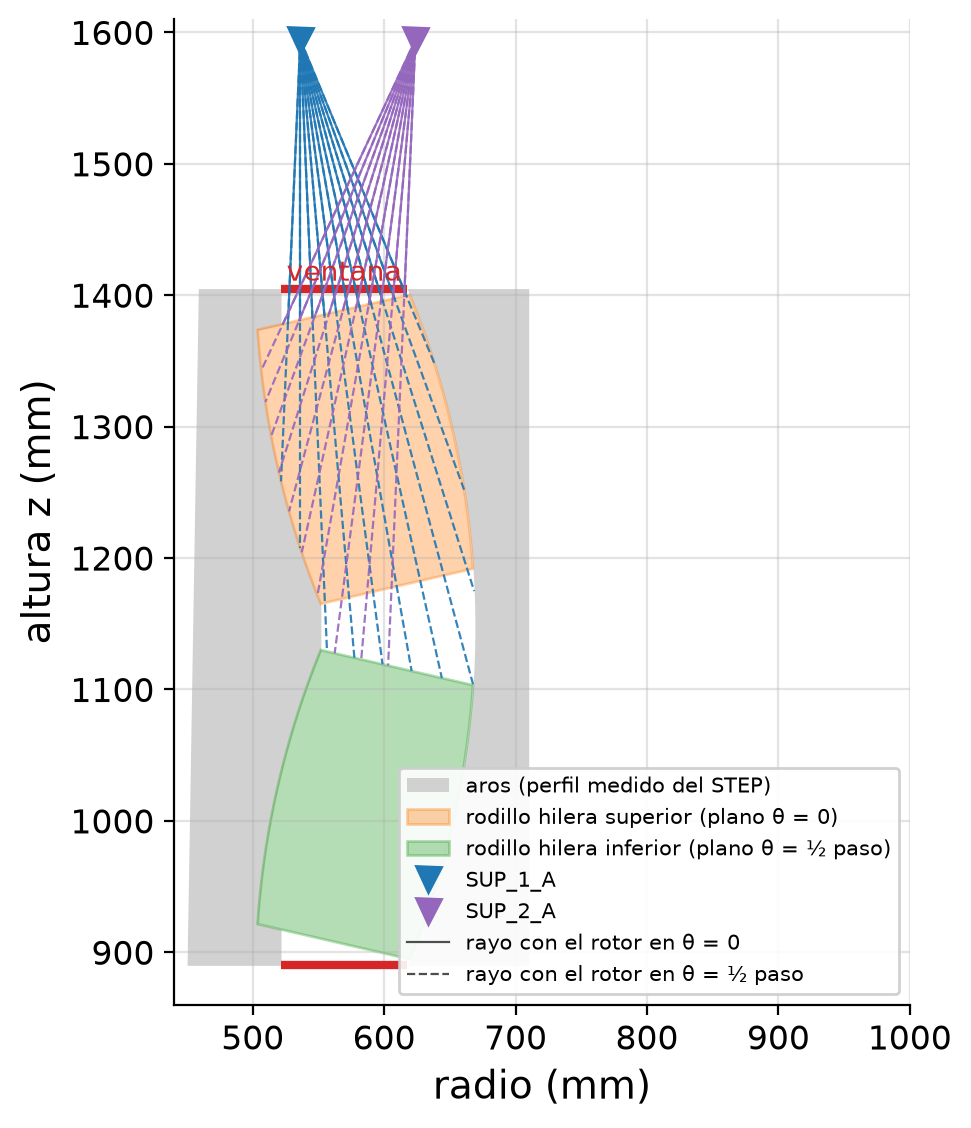
\includegraphics[width=0.55\textwidth]{asp_cavidad_seccion_rayos.png}
\caption[Sección del rodamiento armado con los rayos de las boquillas superiores]{Sección meridiana del rodamiento armado con los rayos de las dos boquillas superiores de un brazo, en dos posiciones del distribuidor. La hilera superior se ve en parte a través de la ventana entre aros y la inferior queda oculta. Geometría medida en el modelo del fabricante, sin jaula. Elaboración propia.}
\label{fig:anx-cavidad}
\end{figure}

\section{Impacto local de un chorro sobre el diámetro exterior}
\label{sec:anx-vof}

El modelo de fase discreta retiene la gota en el primer impacto y no resuelve la película que se forma en la pared. Para estimar la acción hidráulica local se simuló el impacto de la lámina de una boquilla lateral sobre el diámetro exterior con el método de volumen de fluido (VOF) de OpenFOAM v2606 (\texttt{interFoam}), en régimen laminar, con agua a 62~$^\circ$C y aire a 76,24 kPa. El caso es un corte bidimensional a través del espesor de la lámina, de 0,049 mm a 130 mm de la boquilla, con una velocidad de 27,5 m/s y medio dominio con plano de simetría. Se usaron cuatro mallas, con 5, 10, 20 y 40 celdas en el espesor de la lámina, y un número de Courant de 0,5. El orden de convergencia observado fue cercano a 2, la presión de estancamiento quedó dentro del 0,1\,\% de $\tfrac12\rho v^2$ y la fuerza local sobre la pared, un 0,5\,\% por encima de $\rho v^2 e_0$, lo que verifica el modelo frente a la teoría del chorro.

El empuje de la película a 0,33 mm del eje del impacto es de 17,0 N/m por lado, el 94\,\% del valor teórico, y el esfuerzo cortante en la pared en ese punto es de unos 2 kPa, con un pico de unos 9,5 kPa junto al eje (Figura~\ref{fig:anx-vof}). Esos valores suponen que la lámina llega intacta, por lo que son una cota superior. Un segundo caso, tridimensional, con el líquido representado como una mezcla diluida en el volumen del chorro, dio de 5 a 25 Pa, valores que crecen al refinar la malla: es una cota inferior. El esfuerzo cortante real queda entre ambas cotas y depende de si la lámina se rompe en gotas antes de llegar, lo que solo una medición de la huella puede aclarar. Por eso el esfuerzo cortante no se usó como criterio de evaluación del diseño.

\begin{figure}[htbp]
\centering
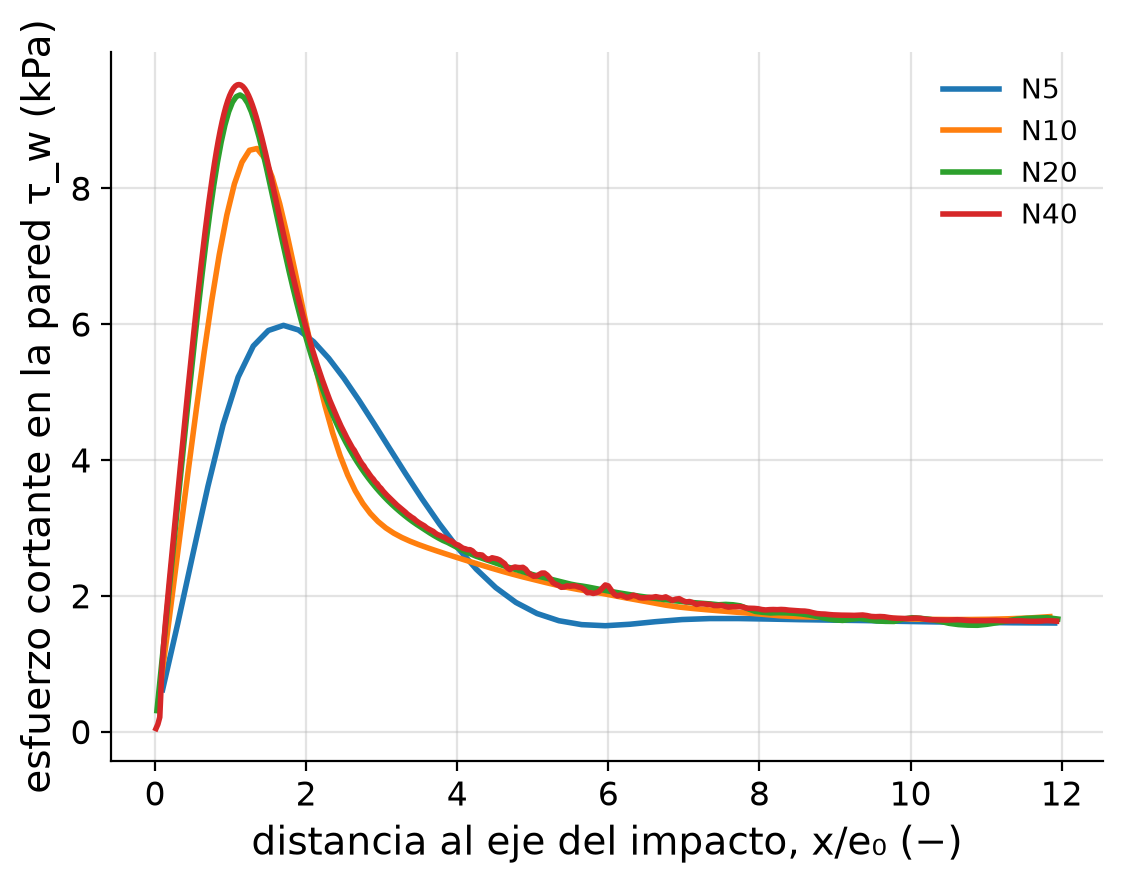
\includegraphics[width=0.58\textwidth]{asp_vof_cortante_od.png}
\caption[Esfuerzo cortante en la pared bajo la lámina de una boquilla lateral]{Esfuerzo cortante en la pared del diámetro exterior bajo la lámina de una boquilla lateral, con cuatro mallas (N5 a N40 celdas en el espesor de la lámina); la distancia al eje del impacto está dividida por el espesor de la lámina, $e_0$. Cota superior: lámina intacta. Elaboración propia, simulación en OpenFOAM v2606.}
\label{fig:anx-vof}
\end{figure}

\section{Correspondencia de nombres de cálculo y archivos}
La Tabla~\ref{tab:correspondencia-sap} relaciona los identificadores que aparecen en los archivos de respaldo con la denominación que se emplea en el informe.

\begingroup
\small\singlespacing
\setlength{\parskip}{0pt}
\setlength{\tabcolsep}{4pt}
\renewcommand{\arraystretch}{1.1}
\begin{longtable}{@{}>{\raggedright\arraybackslash}p{3.6cm}>{\raggedright\arraybackslash}p{\dimexpr(\textwidth-3.6cm-2\tabcolsep)/1\relax}@{}}
\caption{Correspondencia entre identificadores originales y denominaciones del informe}\label{tab:correspondencia-sap}\\
\toprule
\textbf{Denominación} & \textbf{Significado}\\

\midrule\endfirsthead
\caption[]{Correspondencia de identificadores y denominaciones (continuación)}\\
\toprule
\textbf{Denominación} & \textbf{Significado}\\

\midrule\endhead
\midrule\multicolumn{2}{r}{\textit{Continúa en la página siguiente.}}\\\endfoot
\bottomrule\endlastfoot
N3, N4, N5 & Bastidor con tres, cuatro o cinco apoyos sectoriales, respectivamente. Los apoyos reciben el rodamiento y son distintos de las cuatro ruedas del conjunto móvil.\\
R01 & Análisis estructural original realizado en SAP2000.\\
R03, R04, R05 & Revisiones mecánicas: reserva de masa y desarrollo de la integración. R05 identifica la revisión mecánica posterior al análisis original, no cinco apoyos.\\
R06, R06.1 & Integración de la mesa con el aplicador, los rieles y el drenaje (R06) y desarrollo de los centradores K2-M (R06.1). Configuración candidata vigente.\\
\texttt{LC\_G\_FRAME} & Peso propio del bastidor.\\
\texttt{LC\_G\_EXTERNAL} & Carga vertical externa aplicada en los apoyos sectoriales.\\
\texttt{SLS\_NOMINAL} & Combinación nominal de servicio: peso propio y carga externa con factor 1,00.\\
\texttt{SLS\_UNC\_125} & Servicio con carga externa amplificada por 1,25; peso propio con factor 1,00. Este factor no sustituye el factor mecánico 1,15.\\
\texttt{ULS\_1\_4D} & Combinación resistente: factor 1,40 sobre el peso propio y la carga externa, conforme a la Tabla~\ref{tab:combinaciones-r01}.\\
\texttt{DSTL1} & Identificador de la combinación resistente reportada para cuatro y cinco apoyos. Su equivalencia con la combinación del bastidor con tres apoyos no está demostrada.\\
\texttt{Frame}, \texttt{Frames} & Barra o elementos de barra del modelo.\\
\texttt{MatProp = Default} & Campo de asignación del material descrito en el apartado~\ref{sec:material-trazabilidad}. Para el bastidor W6×9 se consideró acero ASTM A36.\\
D/C & Razón demanda/capacidad; no es un factor de seguridad global.\\
PMM & Interacción de carga axial y flexión biaxial.\\
V5.2, I01 & Identificadores de la arquitectura y del cálculo de aspersión documentados.\\
PAD y liner & Apoyo sectorial del rodamiento y revestimiento de su superficie de contacto. En el informe se emplea «apoyos sectoriales».\\
K2-M, v5.7.3, v5.7.4 & Centrador de brazo pivotante de eje vertical derivado del concepto K2. La versión 5.7.3 es la vigente; la 5.7.4 es un estudio de refuerzo no adoptado.\\
U1, U2, U3 & Unidades de centrado: U1 y U3 son las referencias y U2 el empujador.\\
LOAD, WASH & Receptores del pasador de bloqueo en las estaciones de carga y de lavado.\\
E1, E2 & Etapas de limpieza: E1, con el rodamiento montado sobre la mesa, y E2, con sus elementos desmontados.\\
Libro I01 & Identificador documental de la hoja de cálculo hidráulico. En el texto se utiliza «hoja de cálculo hidráulico».\\
\end{longtable}

\endgroup
